% https://de.overleaf.com/learn/latex/How_to_Write_a_Thesis_in_LaTeX_(Part_1)%3A_Basic_Structure
% https://en.wikibooks.org/wiki/LaTeX/Document_Structure
%\documentclass[11pt, twoside]{report}
\documentclass[11pt, a4paper]{report}
%\documentclass[a4paper,11pt]{scrartcl}
\usepackage[utf8]{inputenc}
\usepackage[backend=biber]{biblatex}
\addbibresource{mybib.bib}
\usepackage{hyperref}
\usepackage{graphicx}
\usepackage{color}
\usepackage{framed}
\usepackage{subcaption}
\usepackage{float}
\graphicspath{ {images/} }
\usepackage{blindtext}
\usepackage{mathtools}
\usepackage{amssymb}
\usepackage{amsfonts}
\usepackage{amsthm}
%\usepackage{showframe}
%\usepackage[a4paper, width=150mm, top=5mm, bottom=5mm]{geometry}
\usepackage[a4paper, width=150mm, top=25mm, bottom=25mm]{geometry}
\usepackage{fancyhdr}
\setlength{\headheight}{12pt}
\pagestyle{fancy}
%\pagestyle{empty}
\usepackage{lipsum}

\theoremstyle{plain}
\newtheorem{theorem}{Theorem}[chapter]
\newtheorem{lemma}[theorem]{Lemma}

\theoremstyle{definition}
\newtheorem{mydef}{Definition}[chapter]

\theoremstyle{remark}
\newtheorem{remark}{Remark}[chapter]

\begin{document}
\begin{titlepage}
\begin{center}
{
\includegraphics{images/MPIMG_RGB_gruen.png}}\\
\vspace*{1cm}
%\vfill
\Large
\textbf{List of topics to cover}
%\vfill

%\vspace{0.5cm}


%\normalsize
\large
With section titles and brief explantions.
\vfill
%\vspace{1.0cm}

Yiftach Kolb

Berlin, \today

\vfill
{
\includegraphics{images/fu-logo_bildschirm_RGB1.jpg}}
\end{center}
\end{titlepage}

%\author{Kolb, Yiftach}
%\date{Berlin, \today}
%\title{Topic List}
%\maketitle

\chapter*{Abstract}
punkt.
punkt.
\nocite{guo2017improved}

\chapter*{Declaration}
punkt.
punkt.
\nocite{bishop2006pattern}

\chapter*{Acknowledgement}
punkt.\cite{kingma2013auto}
punkt.

\listoftables

\listoffigures

\tableofcontents

\chapter{Introduction}
punkt.
punkt.

\chapter{Autoencoders, VAEs, and Variance inference}
punkt.
punkt.
\remark{My remark}[See \cite{makhzani2015adversarial}] This is interesting
\dots.
punkt.


\chapter{Gaussian mixture model VAEs}

Theoretical background and 
with some examples from publications and my own tests.


\begin{figure}
\centering
\begin{subfigure}[b]{0.4\textwidth}
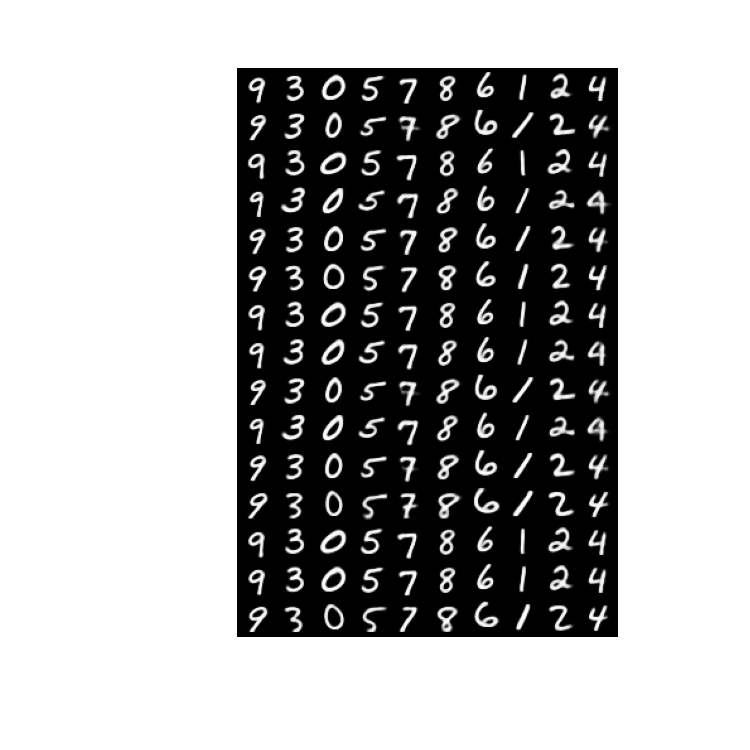
\includegraphics[width=\textwidth]{images/model_mnist_10c_generation.png}
\caption{}
%\caption{blabla}
%\label{bla}
\end{subfigure}
%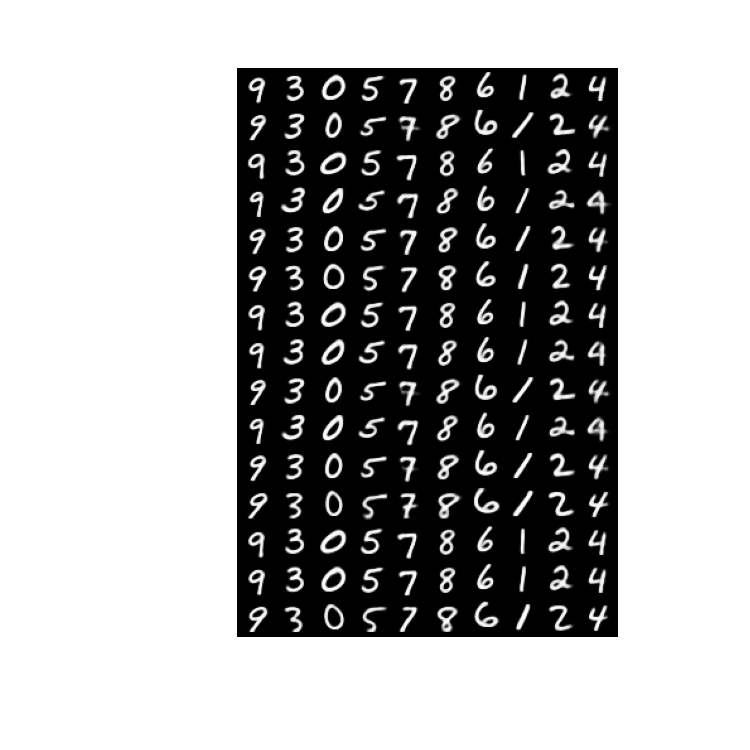
\includegraphics[width=0.4\linewidth]{images/model_mnist_10c_generation.png}
\begin{subfigure}[b]{0.4\textwidth}
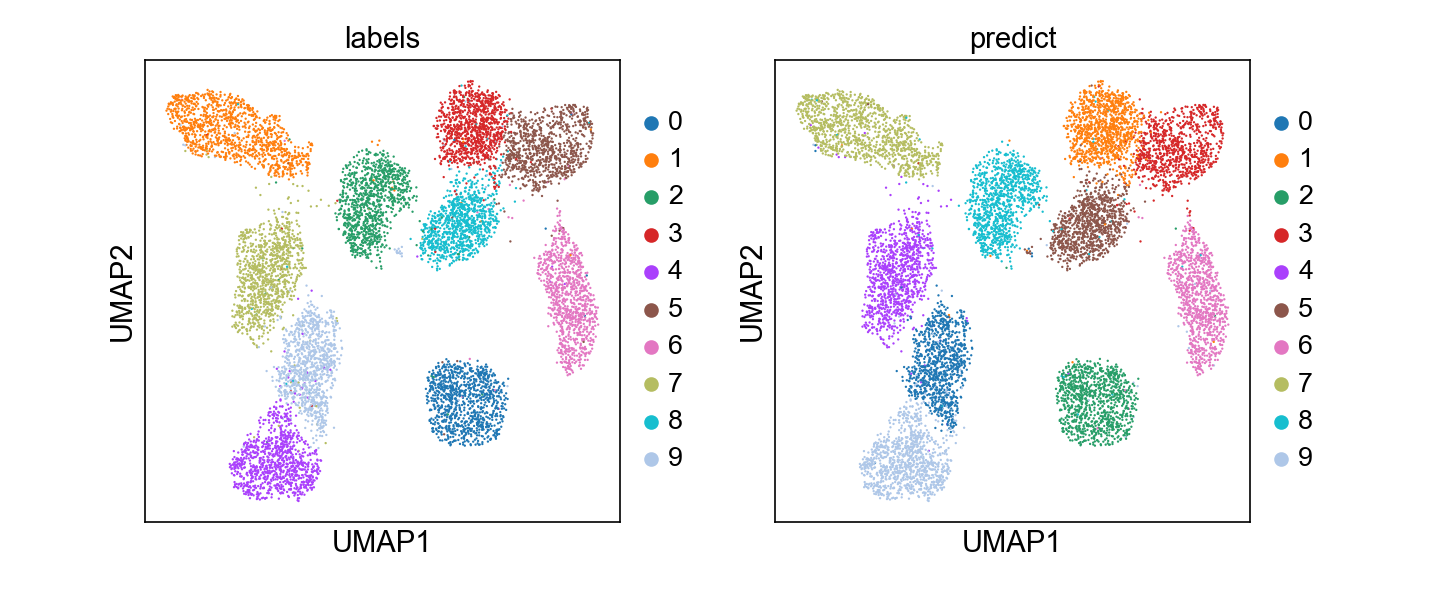
\includegraphics[width=\textwidth]{images/model_mnist_10c_umap.png}
\caption{}
%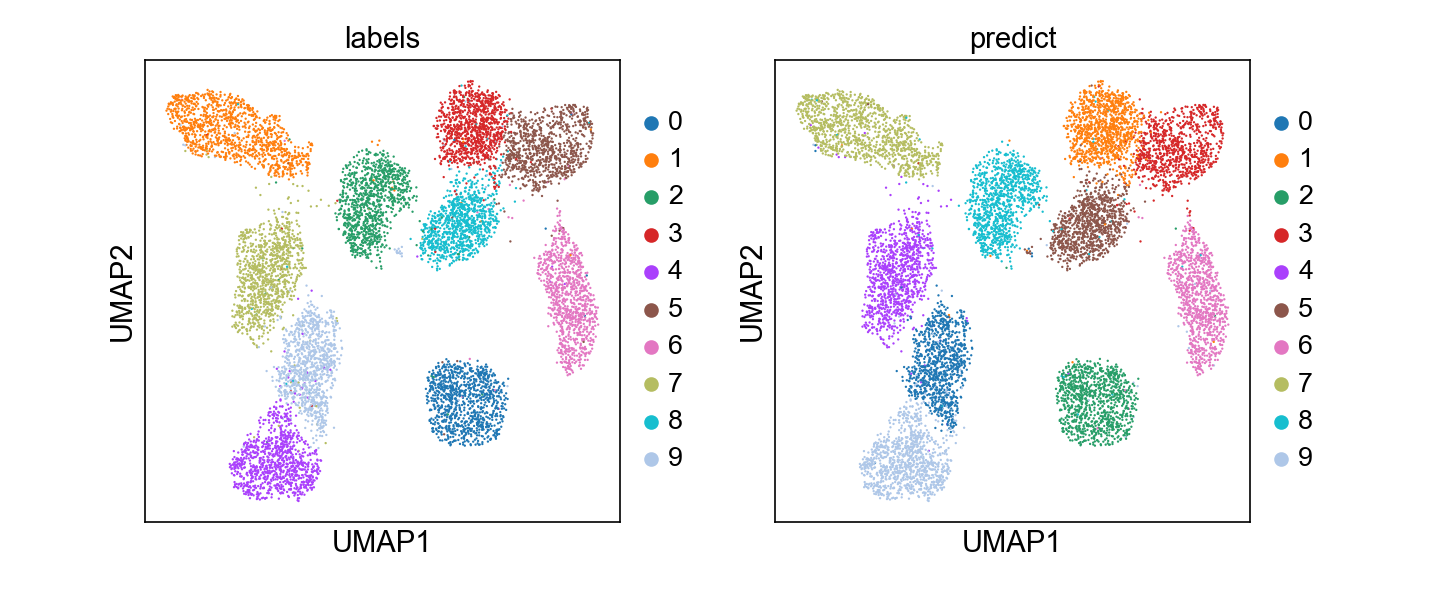
\includegraphics[width=0.4\linewidth]{images/model_mnist_10c_umap.png}
\end{subfigure}
\caption{a figure}
\label{fig:myfig}
\end{figure}

\chapter{Datasets which were tested and results}
some words about (sc)RNAseq and published papers where 
AE and VAE models have been applied.
What we were hoping to achieve and compare with.

\chapter{Discussion, some remarks and conclusions}
punkt.
punkt.
punkt.





%\author{Yiftach Kolb}
%\date{Berlin, \today}
%\maketitle

%\section*{Intro Foo}
%\lipsum{1}
%\section{Bar}
%\lipsum{2}
%\appendix
%\section{Spam}
%\lipsum{3}

\printbibliography

\end{document}


